\documentclass{thesis}
%\usepackage[colorlinks, urlcolor=blue, linkcolor=red, citecolor=red, linktocpage=true]{hyperref}
\usepackage[linktocpage=true]{hyperref}
\usepackage{russianplural}
\usepackage{amsmath}
\usepackage{amssymb}
\usepackage{amsfonts}
\usepackage{totcount}
\usepackage{mdwlist}
\usepackage{makecell}
\usepackage{booktabs}
\usepackage{hyperref}
%\usepackage{showframe}
\usepackage{setspace}
\usepackage{caption}
\usepackage{titlesec}
% \usepackage{float}
\usepackage{listings}
\usepackage{algorithm}
\usepackage[noend]{algpseudocode}
\newcommand{\head}[1]{\textnormal{\textbf{#1}}}

\DeclareMathOperator*{\argmax}{arg\,max}

\makeatletter
\newbox\sf@box
\newenvironment{SubFloat}[2][]%
{\def\sf@one{#1}%
	\def\sf@two{#2}%
	\setbox\sf@box\hbox
	\bgroup}%
{ \egroup
	\ifx\@empty\sf@two\@empty\relax
	\def\sf@two{\@empty}
	\fi
	\ifx\@empty\sf@one\@empty\relax
	\subfloat[\sf@two]{\box\sf@box}%
	\else
	\subfloat[\sf@one][\sf@two]{\box\sf@box}%
	\fi}
\makeatother

% \usepackage{showframe}

\newtotcounter{bibitems}
\setcounter{bibitems}{0}

\captionsetup[subfloat]{farskip=0pt}
% \setlength{\farskip}{0pt}
% \setlength{\textfloatsep}{18pt}

% \setlength{\intextsep}{0pt}

% \setlength{\belowcaptionskip}{-0.5em}

\graphicspath{{pic/}, {pseudocode/}}
\titlespacing{\paragraph}{1.25cm}{1.5em plus .1ex minus .2ex}{1em}
\captionsetup[table]{skip=-0.4em}
\begin{document} % ------------------------------------------------------------
\sloppy

\newpage
\thispagestyle{empty}
\begin{adjustwidth}[]{0cm}{0cm}
\begin{center}
\begin{linespread}{1}


\small{
МИНИСТЕРСТВО ОБРАЗОВАНИЯ И НАУКИ РОССИЙСКОЙ ФЕДЕРАЦИИ\\
Федеральное государственное бюджетное образовательное учреждение\\
высшего образования\\
\textbf{<<Южно-Уральский государственный университет\\
(национальный исследовательский университет)>>\\
Высшая школа электроники и компьютерных наук\\
Кафедра системного программирования}
}

\vspace{\stretch{1}}


{
\large\textbf{Разработка системы для поиска припева в тексте песни}
}

\vspace{2em}

КУРСОВАЯ РАБОТА \\
по дисциплине «Программная инженерия»\\
ЮУрГУ – 09.03.04.2023.308-059.КР


\vspace{\stretch{1}}


\parbox[t]{7cm}{
Нормоконтролер,\\
профессор кафедры СП, д.ф-м.н., \\  
доцент\\[0.5em]
\underline{\hspace{2.5cm}} М.Л.~Цымблер \\[0.5em]
``\underline{\qquad}''\underline{\hspace{2.5cm}} 2024~г.
}
\hfill{}
\parbox[t]{7cm}{
Научный руководитель: \\
профессор кафедры СП, \\
д.ф.-м.н., доцент\\[0.5em]
\underfield{} М.Л.~Цымблер \\[2.5em]
Автор работы, \\
студент группы КЭ-303\\[0.5em]
\underfield{} А.А.~Летуновский \\[2.5em]
Работа защищена \\
с оценкой: \underfield{} \\[0.5em]
``\underline{\qquad}''\underfield{} 2024~г.
}

\vspace{\stretch{1}}

Челябинск 2024

\end{linespread}
\end{center}
\end{adjustwidth}

\pagebreak
 % титульный лист

% \thispagestyle{empty}
\setcounter{page}{2}
\newpage
\thispagestyle{empty}

\begin{adjustwidth}{-1.5cm}{0.5cm}
\begin{linespread}{1}
\begin{center}


\small{
МИНИСТЕРСТВО ОБРАЗОВАНИЯ И НАУКИ РОССИЙСКОЙ ФЕДЕРАЦИИ\\
Федеральное государственное бюджетное образовательное учреждение\\
высшего образования\\
\textbf{<<Южно-Уральский государственный университет\\
(национальный исследовательский университет)>>\\
Высшая школа электроники и компьютерных наук\\
Кафедра системного программирования}
}



\vspace{2em}

\hfill{}
\parbox{7cm}{
УТВЕРЖДАЮ \\
Зав. кафедрой СП \\[0.5em]
\underfield{} Л.Б.~Соколинский \\[0.5em]
"\underline{\qquad}"\underfield{}2024
}

\vspace{2em}

\textbf{ЗАДАНИЕ} \\
% \parbox[t]{14cm}{
\textbf{на выполнение выпускной курсовой работы}\\
студенту группы КЭ-303\\
Летуновскому Арсению Александровичу,\\
обучающемуся по направлению 09.03.04 «Программная инженерия» 
% }

\end{center}

\vspace{2em}

{
\small
\begin{enumerate}
	\bf\item Тема работы \rm
	(утверждена приказом ректора от  \No~)\\
	Разработка системы для поиска припева в тексте песни

	\bf\item Срок сдачи студентом законченной работы: \rm
	31.05.2024~г.

	\bf\item Исходные данные к работе\rm
	\begin{enumerate}%[leftmargin=0.35cm]
		\raggedright

		\item Imani, S., Madrid, F., Ding, W. et al. Introducing time series snippets: a new primitive for summarizing long time series // Data Min Knowl Disc 34, 2020. --P. 1713–-1743.

        \item Watanabe K., Goto M. A Chorus-Section Detection Method for Lyrics Text. // Proceedings of the 21th International Society for Music Information Retrieval Conference, {ISMIR} 2020, Montreal, Canada, October 11--16, 2020. --P 351–359

	\end{enumerate}

	\bf\item Перечень подлежащих разработке вопросов\rm
	\begin{enumerate}
		\item Выполнить анализ предметной области и провести обзор существующих решений.
		\item Выполнить разработку алгоритма поиска припева в тексте песни на основе поиска типичных подпоследовательностей временного ряда. 
		\item Разработать приложение для использования алгоритма поиска припева в тексте песни.
		\item Разработать тестовые наборы и провести тестирование разработанного приложения.
        \item Оценить точность полученных результатов относительно истинной разметки.
	\end{enumerate}

	\bf\item Дата выдачи задания: \rm
	"\underline{\qquad}"\underfield{}2024~г.
\end{enumerate}

\vspace{1em}

\noindent
\textbf{Научный руководитель}
\hfill
\hbox to 8em{М.Л.~Цымблер\hfill}

\vspace{1em}

\noindent
\textbf{Задание принял к исполнению}
\hfill
\hbox to 8em{A.А.~Летуновский\hfill}

}

\thispagestyle{empty}

\end{linespread}
\end{adjustwidth}

\pagebreak


\newpage
%{\linespread{1.1}
\tableofcontents % оглавление
%}

\newpage
\sectionnonumber{Введение}
\subsection*{Актуальность темы}
Описание причин создания данного проекта.
\subsection*{Цель и задачи исследования}
Целью данной курсовой работы является разработка системы поиска припева в тексте песни.

Для достижения поставленной цели необходимо решить следующие задачи:
\begin{enumerateparen}
    \item Провести обзор аналогичных проектов.   
    \item Выполнить разработку алгоритма классификации припевов и куплетов.
    \item Разработать приложения для разметки текстов песен, настройки и запуска алгоритмов, анализа результатов и визуализации данных.
    \item Провести разметку песен и составить из них набор данных.
    \item Провести тестирование разработанного алгоритма.
\end{enumerateparen}
\subsection*{Структура и объем работы}
\newcounter{biconvert}
\setcounter{biconvert}{\totvalue{bibitems}}
\regtotcounter{chapter}
Курсовая работа состоит из введения, четырех глав, заключения и библиографического списка. Объем работы составляет \numplural{\getpagerefnumber{LastPage}}{страниц}{страницу}{страницы}, объем списка литературы~-- \numplural{\arabic{biconvert}}{наименований}{наименование}{наименования}.
\subsection*{Содержание работы}
Первая глава, <<АНАЛИЗ ПРЕДМЕТНОЙ ОБЛАСТИ>>, содержит обзор предметной области, а так же анализ существующих решений по тематике курсовой работы.

Во второй главе, <<ПРОЕКТИРОВАНИЕ>>, содержатся функциональные и нефункциональные 
требования к разрабатываемому приложению. Приведены варианты использования программы, архитектура приложения, его компоненты и пользовательский интерфейс.

Третья глава, <<РЕАЛИЗАЦИЯ>>, содержит описание программных средств, используемых в процессе реализации системы, описание реализации алгоритма поиска припева песни, а также пользовательского интерфейса.

В четвертой главе, <<ТЕСТИРОВАНИЕ>>, представлено функциональное тестирование и оценка точности полученных результатов относительно истинной разметки.

В заключении подведены основные итоги выполненной работы.
\newpage
\section{Анализ предметной области}
\label{sec:Background}

\subsection{Описание предметной области}
Обзор временных рядов, сниппетов временных рядов, а также алгоритмов поиска данных сниппетов во временном ряде.
\vspace{2em}
\subsection{Анализ аналогичных проектов}
Работ со схожей тематикой немного. Наиболее близким аналогом является работа японских исследователей\cite{WatanabeG20}, в которой для выделения из текста песни куплетов и припевов используется модель, основанная на обученной нейронной сети. Данная нейронная сеть анализирует девять матриц самоподобия, составленных на основе текста песни.

После того как были созданы матрицы самоподобия, высчитываются векторы признаков с помощью сверточной нейронной сети. Данные векторы используются двунаправленными сетями с длительной кратковременной памятью для разметки текста песни.


Анализ текста используется не только для выделения припевов и куплетов, но также для распознавания жанра песни, как в работе австрийских исследователей\cite{Genre}. В данной работе предложено создание набора десяти различных признаков на основе текста песни и последующий их анализ с помощью алгоритмов классификации, таких как: случайный лес, метод опорных векторов и нейронной сети с прямой связью.


Еще одним способом выделения куплетов и припевов является анализ звуковых дорожек песен. Данный способ является более исследованным, чем анализ текста.

Например, модель "DeepChorus"\cite{DeepChorus}, которая использует сочетание многомасштабной сверточной сети для получения предварительной разметки и self-attention сверточной нейронной сети для обработки признаков в кривые вероятности, представляющие присутствие припева. Чтобы получить окончательные результаты, применяется адаптивный порог для бинаризации исходной кривой.

Другая модель "LA-Chorus"\cite{LA-Chorus} основана на увеличении скрытых функций и архитектуре ResNetFPN. Во-первых, предлагается метод неявного увеличения данных припева в скрытом пространстве на этапе обучения. Во-вторых, применяется нейронная сеть (FPN) для генерации дополнительных признаков от низкой размерности к высокой размерности, достигая многомасштабной парадигмы обучения. 

Модель "MMCR" (Multi-Modal Chorus Recognition)\cite{MMCR} анализирует одновременно и текс песни, и аудиосигнал. Каждой строке текста ($S_i$) сопоставлена часть аудиосигнала ($A_i$). Информация о $A_i$ представляется в виде мел-кепстральные коэффициентов (MFCC). Информация о $S_i$ получается с помощью
предварительно обученной языковой модели и графовой нейронной сети (Graph Attention Networks). После получения конечной характеристики $F_i$, основанной на соответствующей информации о тексе и аудиосигнале, используется классификатор, чтобы предсказать, принадлежит ли ($A_i$, $S_i$) припеву.

В следующей работе\cite{ByteDance} так же используется сверточная нейронная сеть. На вход данной нейронной сети поступает мел-спектрограмма песни. После обработки данных нейронной сетью необходимо так же как и в модели "DeepChorus"\cite{DeepChorus} происходит бинаризация полученных результатов. Конечные данные показывают, к какому разделу песни относится каждый из отрывков.

Выделение одних частей звукового сигнала от других используется не только для разделения песни на припевы и куплеты, но и применяется в других сферах деятельности человека. Так, например, основанный на энтропии подход\cite{Fish} помогает выделять звуки, издаваемые рыбами, среди всех остальных антропогенных шумов. Благодаря этому имеется возможность точно оценить популяцию исследуемых рыб.



\newpage
\section{Проектирование}
\label{sec:Definition}
 
\subsection{Требования к системе}
\textbf{Функциональные требования.}

Функциональные требования определяют действия, которые должна выполнять программа.

\textbf{Нефункциональные требования.}

Нефункциональные действия определяют свойства программы (удобство использования, безопасность и т.д.). 
\vspace{2em}
\subsection{Варианты использования системы}
Описать, как пользователь может работать с приложением.
\vspace{2em}
\subsection{Архитектура приложения}
Определить из каких модулей будет состоять приложение, а также описать функционал каждого из них.
\vspace{2em}
\subsection{Графический интерфейс}
Описать, как будет выглядеть графический интерфейс приложения. Сделать макеты.
% Formatting of listings
\lstset{language=C, frame=L, basicstyle=\footnotesize,%\sffamily,
	keywordstyle=\bfseries, showstringspaces=false, xleftmargin=\parindent, numbers=none, numberstyle=\tiny, stepnumber=2, numbersep=5pt}
\newpage
\section{Реализация}
\label{sec:Design}
\subsection{Программные средства реализации}
Для разработки программной части приложения использовался высокоуровневый язык программирования Python версии 3.9.18. Программирование осуществлялось в интегрированной среде разработки PyCharm Community 2023.3.4~\cite{pycharm}.
\vspace{2em}
\subsection{Реализация компонентов приложения}
Описать работу каждого модуля, входные и выходные данные, вставить код.


\vspace{2em}
\subsection{Реализация пользовательского интерфейса}
Реализация пользовательского интерфейса осуществлялась на основе разработанных макетов. Реализованы окна главного меню, разметки песен и визуализации результатов. В качестве основы разработки интерфейса использовалась библиотека tkinter~\cite{tkinter}.

\begin{figure}
    \centering
    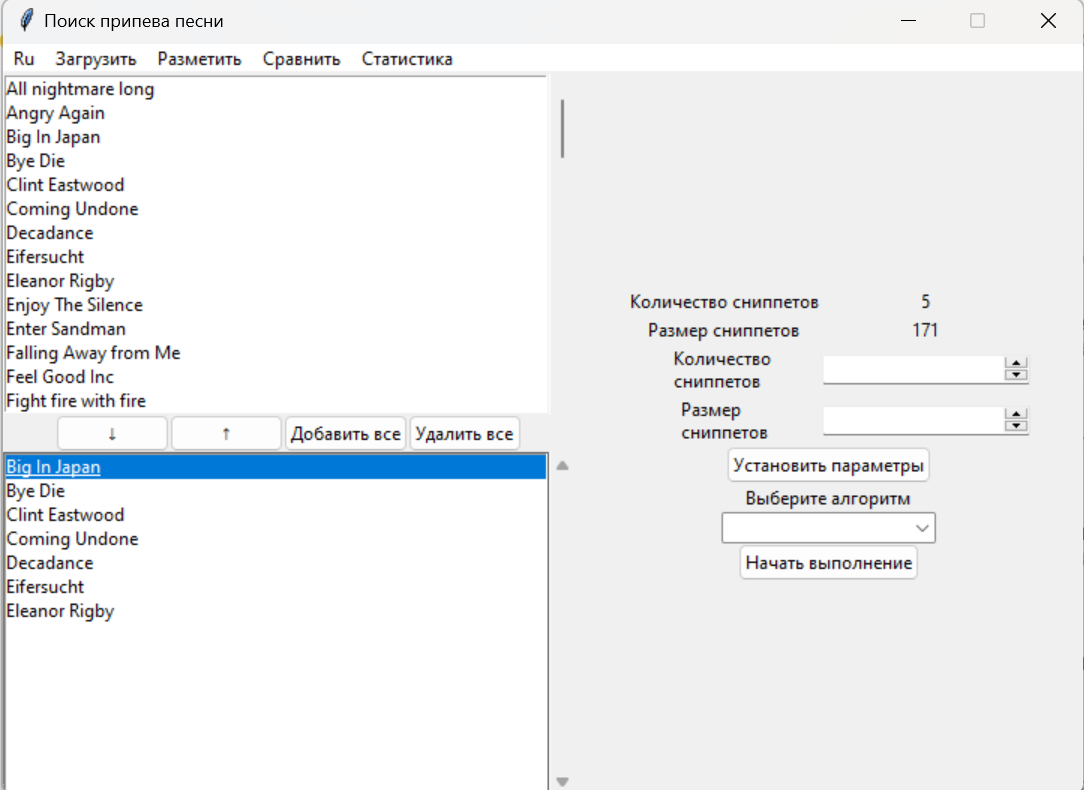
\includegraphics[width=1\linewidth]{pictures/Главный_скрин.png}
    \caption{Окно главного меню}
    \label{fig:Главный_скрин}
\end{figure}

На рисунке~\ref{fig:Главный_скрин} представлено главное окно приложения. Оно содержит два списка песен, два поля для просмотра параметров песни, два поля для ввода числовых значений, кнопку для сохранения введённых параметров, выпадающий список с выбором алгоритма классификации и кнопку начала работы. Кроме того, главное окно имеет верхнее меню, в котором можно сменить язык с русского на английский, загрузить тексты песен в приложение, открыть окно разметки и открыть окно визуализации результатов.

\begin{figure}
    \centering
    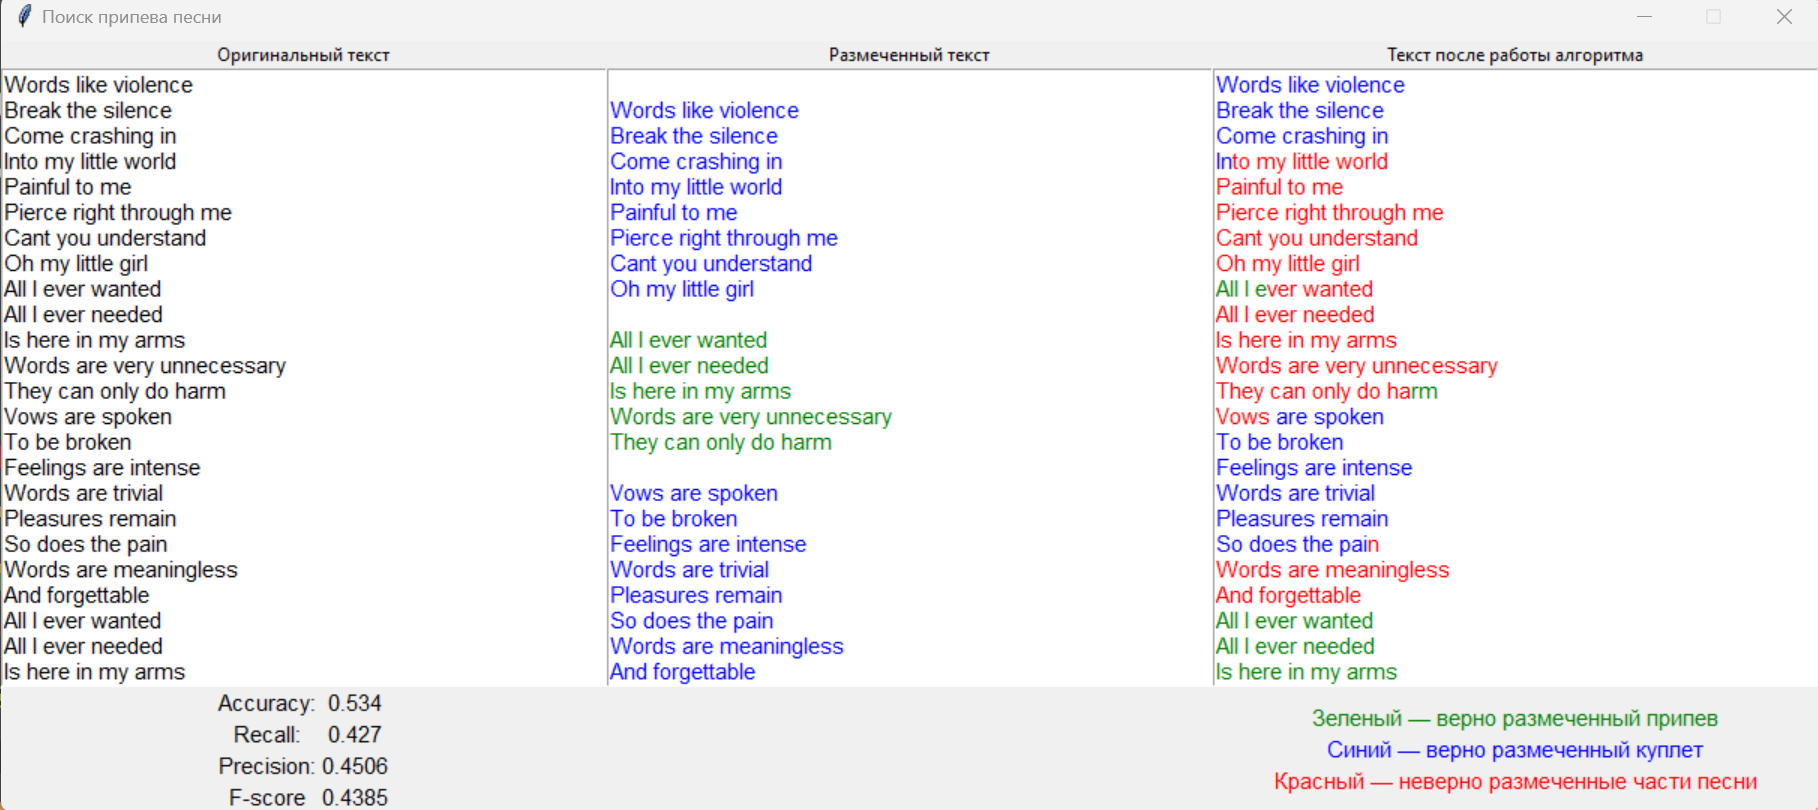
\includegraphics[width=1\linewidth]{pictures/Результаты_скрин.png}
    \caption{Окно визуализации результатов}
    \label{fig:Результаты_скрин}
\end{figure}

На рисунке~\ref{fig:Результаты_скрин} представлено окно визуализации результатов. Оно содержит три текстовых поля с текстом песни, метрики, такие как accuracy, precision, recall и F-score.
\newpage
\section{ТЕСТИРОВАНИЕ}
\label{sec:Experiments}

\subsection{Функциональное тестирование}
Проверка соответствия функциональным требованиям
\vspace{2em}

\subsection{Оценка точности полученных результатов относительно истинной разметки}
Придумать и описать метрики для оценки полученных результа-тов
\newpage
\sectionnonumber{Заключение}
Выводы о проделанной работе.


\newpage
{\raggedright
\phantomsection\addcontentsline{toc}{section}{\refname}
\bibliographystyle{ugost2008}
\bibliography{thesis}
}
% \printbibliography[env=gostbibliography, sorting=ntvy]

\end{document}

% vim: set tw=72 syntax=tex:
